%basic_buried_waveguide
In agreement with the waveguide in the experiment, the buried waveguide model likes Fig. \ref{fig:buried_waveguide} is created with the same corresponding parameters. The waveguide in this section contains the identical dimensions ($w$ and $h$) and refractive indexes (n$_{1}$ and n$_{2}$) with the original waveguide. 
\begin{figure}[!ht]
\centering
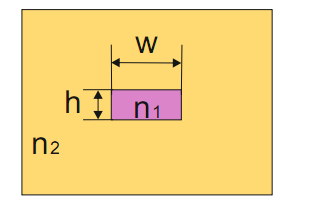
\includegraphics[width=0.6\textwidth]{bilder/buried_waveguide}
\caption{Schema of a basic buried waveguide}
\label{fig:buried_waveguide}
\end{figure}
Fig. \ref{fig:curve_coupling_basic_buried_waveguide} shows the coupling efficiency between TLF and the basic buried waveguide due to the frequencies. The coupling efficiency at the working frequency $282$THZ reaches about $51.3\%$, which is relative better than stripped rib waveguide. We will refer this value for further discussion about coupling between TLF and the lensed waveguide.  
\begin{figure}[!ht]
\centering
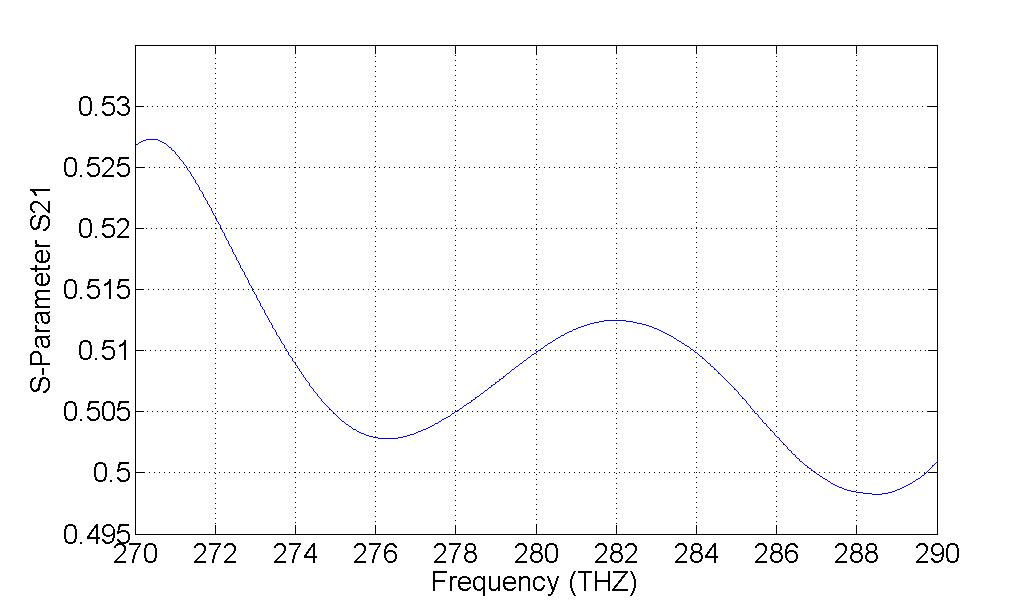
\includegraphics[width=0.8\textwidth]{bilder/s21_sym_waveguide}
\caption{Coupling efficiency curve between TLF and the basic buried waveguide due to frequency domain.}
\label{fig:curve_coupling_basic_buried_waveguide}
\end{figure}
